\section{Background}
\label{sec:bg}

MRIS is a key/value store designed for multi-resolution image
workloads using a multi-tier architecture consisting of Flash SSD and
magnetic HDD.

\subsection{Flash SSD}
Flash is a type of non-volatile memory. There are two main types of
flash memory, which are named after the NAND and NOR logic
gates~\cite{flashwiki}. NAND is the more popular one used in
SSDs~\cite{ssdanatomy}.  NAND flash chip is able to trap electrons
between its gates. The absence of electrons corresponds to a logical
0. Otherwise, it corresponds to a logical 1. NAND can be furthered
divided into SLC and MLC by the number of bits can be represented in a
cell.

NAND Flash has asymmetric read and write performance. Read is fast and
takes roughly 50$mu$s for a MLC~\cite{ssdanatomy}. Write is 10-20
times slower than read. However, write is complicated in the sense
that bits cannot be simply overwritten. Before writes, a block has to
undergo an erase procedure which is 2-3 order of magnitude slower than
read. Moveroever, NAND Flash cell can endure only limit cycles of
erasing. Therefore, Flash chips are often used for storage in the form
of SSD, which also contains internal controller, processor and RAM.
Algorithms including log-structured writing, wear-leveling, and
garbage collection are implemented inside SSD to make Flash writes
faster and endures longer.

\subsection{Key/Value Store}
We implemented MRIS using LevelDB~\cite{leveldb-web}, an open source
key/value database engine developed by Google.  LevelDB is
log-structured and organizes data into Sorted String Table (SSTable).
SSTable, introduced in Bigtable~\cite{chang06osdi}, is an immutable
data structure containing a sequence of key/value pairs sorted by the
key as shown in Figure~\ref{fig:sstable}. Besides key and value, there
might be optional fields such as CRC, compression type etc. SSTable
are mostly saved as files and each of them can contains data
structures, such as bloomfilter, to facilitate key lookup. SSTable
have counterpart in the memory called Memtable. The key/value pairs in
Memtable are often kept in data structures easy for insert and lookup
such as red/black tree and skiplist.

LevelDB, as well as most other key/value engines, use Log-Structured
Merge Trees (LSM)~\cite{lsm} for internal storage. When key/value
pairs are first added, they are inserted into Memtable.  Once the size
of the Memtable growes beyond a certain threshold, the whole Memtable
is flushed out into a SSTable, and a new Memtable is created for
insertion. When key/value pairs get changed, the new pairs are
inserted without modifying the old pairs. When a key/value pair is
deleted, a marker of the deletion is inserted by setting a flag inside
the key called \texttt{KeyType}. This way key/value can provide large
insertion throughput because data is written out using sequential
I/Os, which have good performance on Hard Disk Drives (HDD). 

\begin{figure}[t]
\begin{centering}
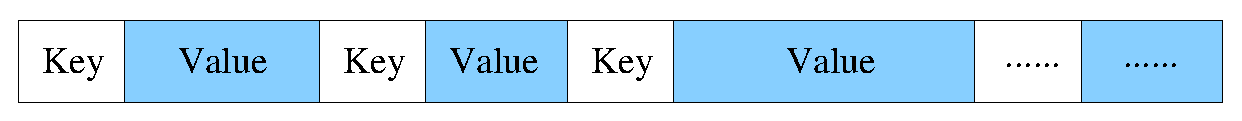
\epsfig{file=figures/sstable.eps,width=1.00\linewidth}
\caption{SSTable}
\label{fig:sstable}
\end{centering}
\end{figure}

\begin{figure}[t]
\begin{centering}
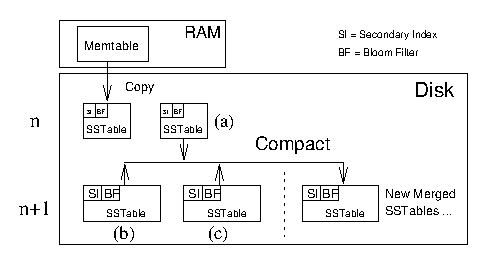
\epsfig{file=figures/leveldb-compact.eps,width=1.00\linewidth}
\caption{LevelDB Compaction}
\label{fig:compact}
\end{centering}
\end{figure}

To serve a key lookup, Memtable is queried firstly. If not found in
Memtable, the SSTables are queried in reverse chronological order. A
naive implementation of such a lookup can be very slow because the
whole database need be read and checked in the worst case. To make
lookup fast, SSTable are organized into several layers with the size
of each table increasing from the top layer to the bottom. Background
jobs are launched periodically to sort and merge small SSTables into
larger ones in the next layer. This is called compaction. Deleted
pairs are also removed during compaction. Then a lookup iterates the
SSTables layer by layer and returns once the key is found.  Because
SSTables are sorted by key, it enables fast lookup algorithm like
binary search. There is also index for SSTables tells the key range
covered by a particular SSTable so that it suffice just checking the
SSTables whose key ranges cover the interested key. Inside each
SSTable, we can have a bloomfilter to filter negative key lookup and a
secondary index for faster search.

In LevelDB, there are two Memtables, once one is filled, the other one
is used for further insertion. The filled one is flushed into a
Memtable in background. Its compaction procedure is illustrated in
Figure~\ref{fig:compact}. One SSTable (a) at layer $n$ is merged with
the SSTables at layer $n+1$ that have overlapping keys with (a) into
new SSTables at layer $n+1$.

%Background...

%Typical length: 0 pages to 1.0.

%Background and Related Work can be similar.
%Most citations will be in this section.

%1. Describe past work and criticize it, fairly.  Use citations
   %to JUSTIFY your criticism!  Problem: hard to compare to YOUR
   %work, b/c you've not yet described your work in enough
   %detail.  Solution: move this text to Related Work at end of
   %paper.

%2. Describe in some detail, background material necessary to
   %understand the rest of the paper.  Doesn't happen often,
   %esp. if you've covered it in Intro.

%Example, submit a paper to a storage conference: reviewers are
%experts in storage.  Don't need to tell them about basic disk
%operation.  But if your paper, say, is an improvement over an
%already-advanced data structure (eg., COLA), then it'd make
%sense to describe basic COLA algorithms in some detail.

%Important: open the bg section with some "intro" text to tell
%reader what to expect (so experienced readers can skip it).

%If your bg material is too short, can fold it into opening of
%'design' section.


%\textbf{notes about picking a project}

%Put every possible related citation you can! (esp. if conf.
%doesn't count citations towards page size).

%Literature survey:
%- CiteSeer

%- Google Scholar

%- libraries

%1. find a few relates paper

%2. skim papers to find relevance

%3. search for add'l related papers in Biblio.

%4. reverse citation: use srch engines, to find
   %newer papers that cite the paper you like.

%5. "stop" when reach transitive closure

%- then go off and read it.

%- think about "how can I improve" and "what was so
  %good about that paper".

%- check future work for project ideas.

%- go to talks \& conferences

%Pick an idea:

%- novelty vs. incremental (how big of an increment?)

%- idea vs. practical implications
  %(implemented? released? in use as OSS or commercial?)

%- where to submit? good fit and match for quality.

%- look at schedule of conferences: due dates \& result dates.

%%%%%%%%%%%%%%%%%%%%%%%%%%%%%%%%%%%%%%%%%%%%%%%%%%%%%%%%%%%%%%%%%%%%%%%%%%%%%%
%% For Emacs:
% Local variables:
% fill-column: 70
% End:
%%%%%%%%%%%%%%%%%%%%%%%%%%%%%%%%%%%%%%%%%%%%%%%%%%%%%%%%%%%%%%%%%%%%%%%%%%%%%%
%% For Vim:
% vim:textwidth=70
%%%%%%%%%%%%%%%%%%%%%%%%%%%%%%%%%%%%%%%%%%%%%%%%%%%%%%%%%%%%%%%%%%%%%%%%%%%%%%
% LocalWords:  SMR HDDs drive's SMRs
